% Author: Victor Terron (c) 2013
% Email: `echo vt2rron1iaa32s | tr 132 @.e`
% License: CC BY-SA 4.0

\begin{frame}{6. El módulo antigravedad}
  \Large
  \begin{block}{}
    \centering import antigravity
  \end{block}{}

  \begin{figure}
    \centering
    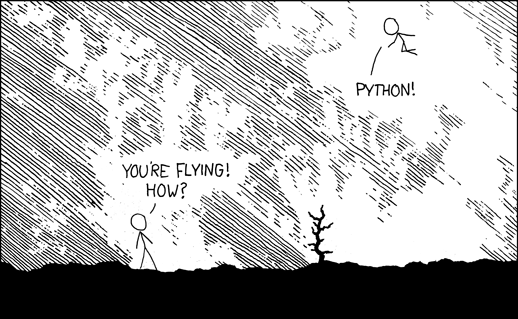
\includegraphics[height=4cm]{pics/xkcd-353.png}
    \caption{\url{http://xkcd.com/353/}}
  \end{figure}

  \small
  \begin{alertblock}{}
    \centering
    Añadido en Python 3, pero también está disponible en Python 2.7
  \end{alertblock}
\end{frame}

\begin{frame}[fragile]{6. El módulo antigravedad}
  \begin{exampleblock}{\small antigravity.py}
    \small
    \begin{lstlisting}
>>> print inspect.getsource(antigravity)
import webbrowser
webbrowser.open("http://xkcd.com/353/")
    \end{lstlisting}
  \end{exampleblock}

  \begin{center}
     \small
     En Py3K el módulo \structure{antigravity} incluye la función
     \structure{geohash()}, referencia a otra viñeta de XKCD en la que
     se describe un algoritmo que genera coodenadas en base a la fecha
     y tu posición actual: \url{http://xkcd.com/426/}
  \end{center}

  \small
  \begin{block}{\centering The History of Python - import antigravity}
    \centering
    \scriptsize
    \url{http://python-history.blogspot.com.es/2010/06/import-antigravity.html}
  \end{block}
\end{frame}
